%%%%%%%%%%%%%%%%%%%%%%%%%%%%%%%%%%%%%%%%%%%%%%%%%%%%%%%%%%%%%
\section{Docker Image for Oscillating Neutrino Spectra}\label{sec:apdx_nu_spec}
%%%%%%%%%%%%%%%%%%%%%%%%%%%%%%%%%%%%%%%%%%%%%%%%%%%%%%%%%%%%%
\lstinputlisting[language=bash]{appendices/Dockerfile.txt}

\clearpage

%%%%%%%%%%%%%%%%%%%%%%%%%%%%%%%%%%%%%%%%%%%%%%%%%%%%%%%%%%%%%
\section{Spline Fitting Statuses} \label{sec:apdx_nu_splines}
%%%%%%%%%%%%%%%%%%%%%%%%%%%%%%%%%%%%%%%%%%%%%%%%%%%%%%%%%%%%%

\begin{figure}[ht]
    \centering{
        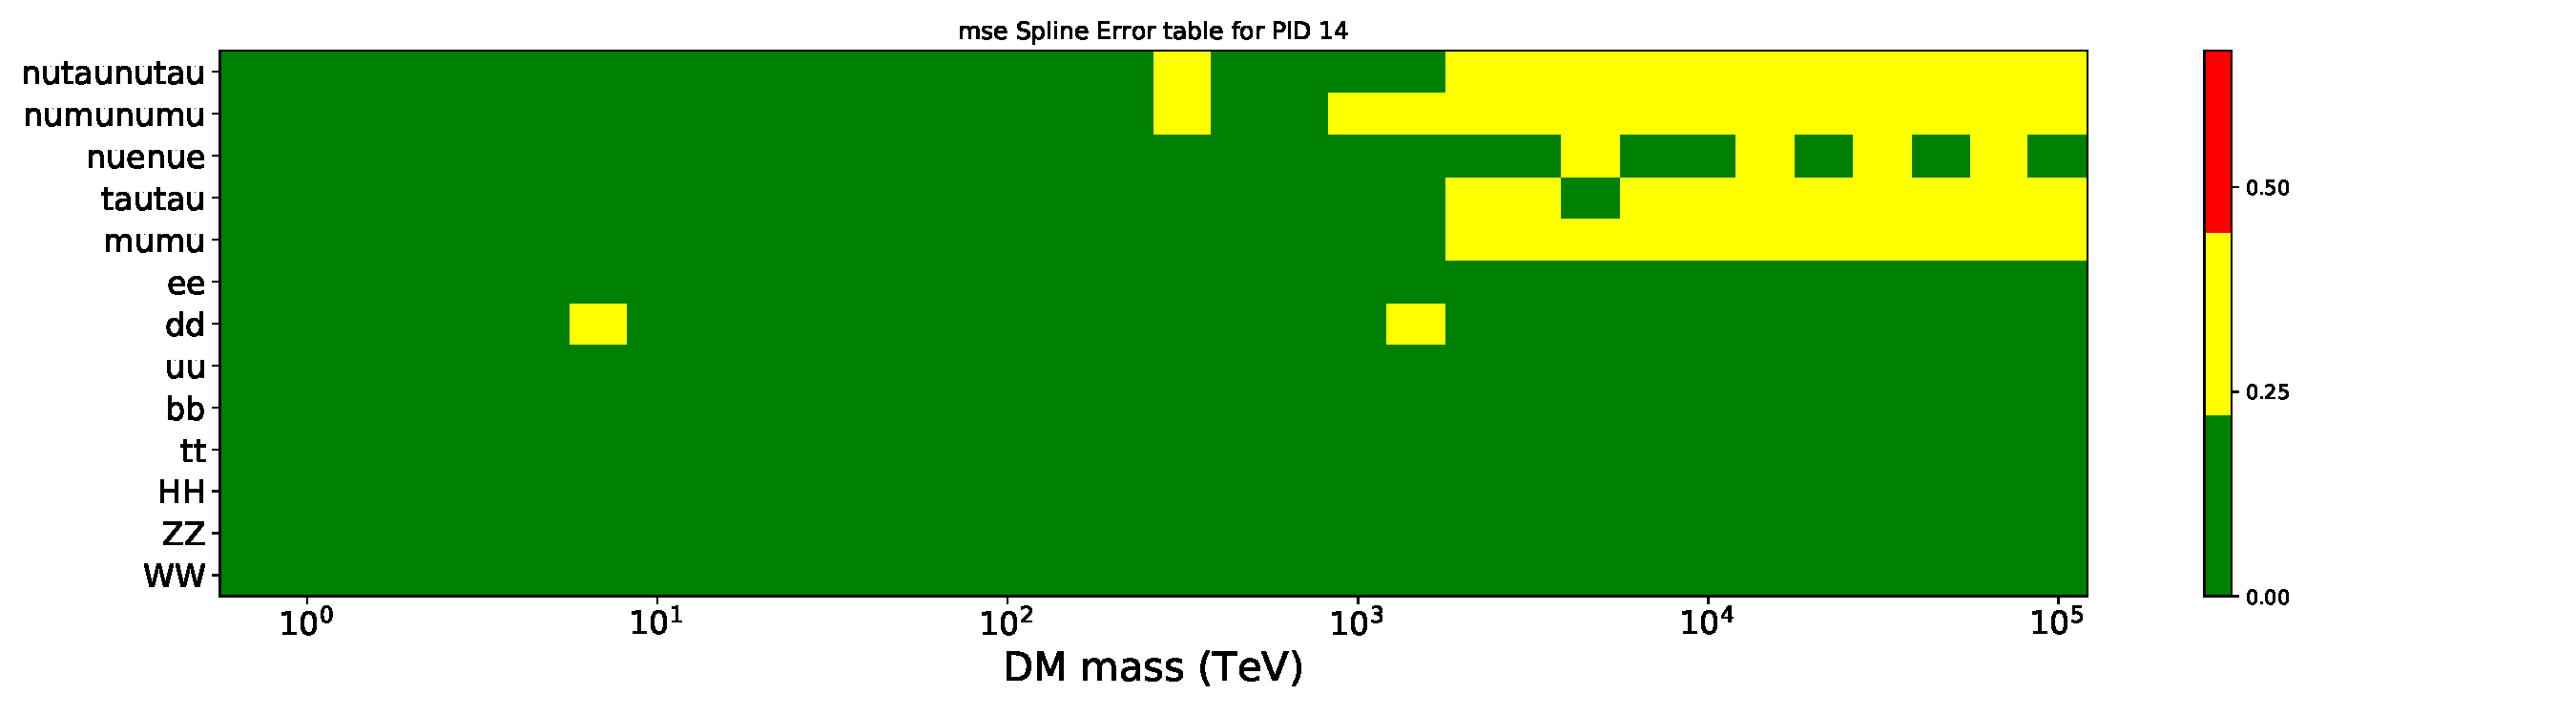
\includegraphics[scale=0.32]{figures/ic_DM/PID14_mse_error_chart.pdf}
        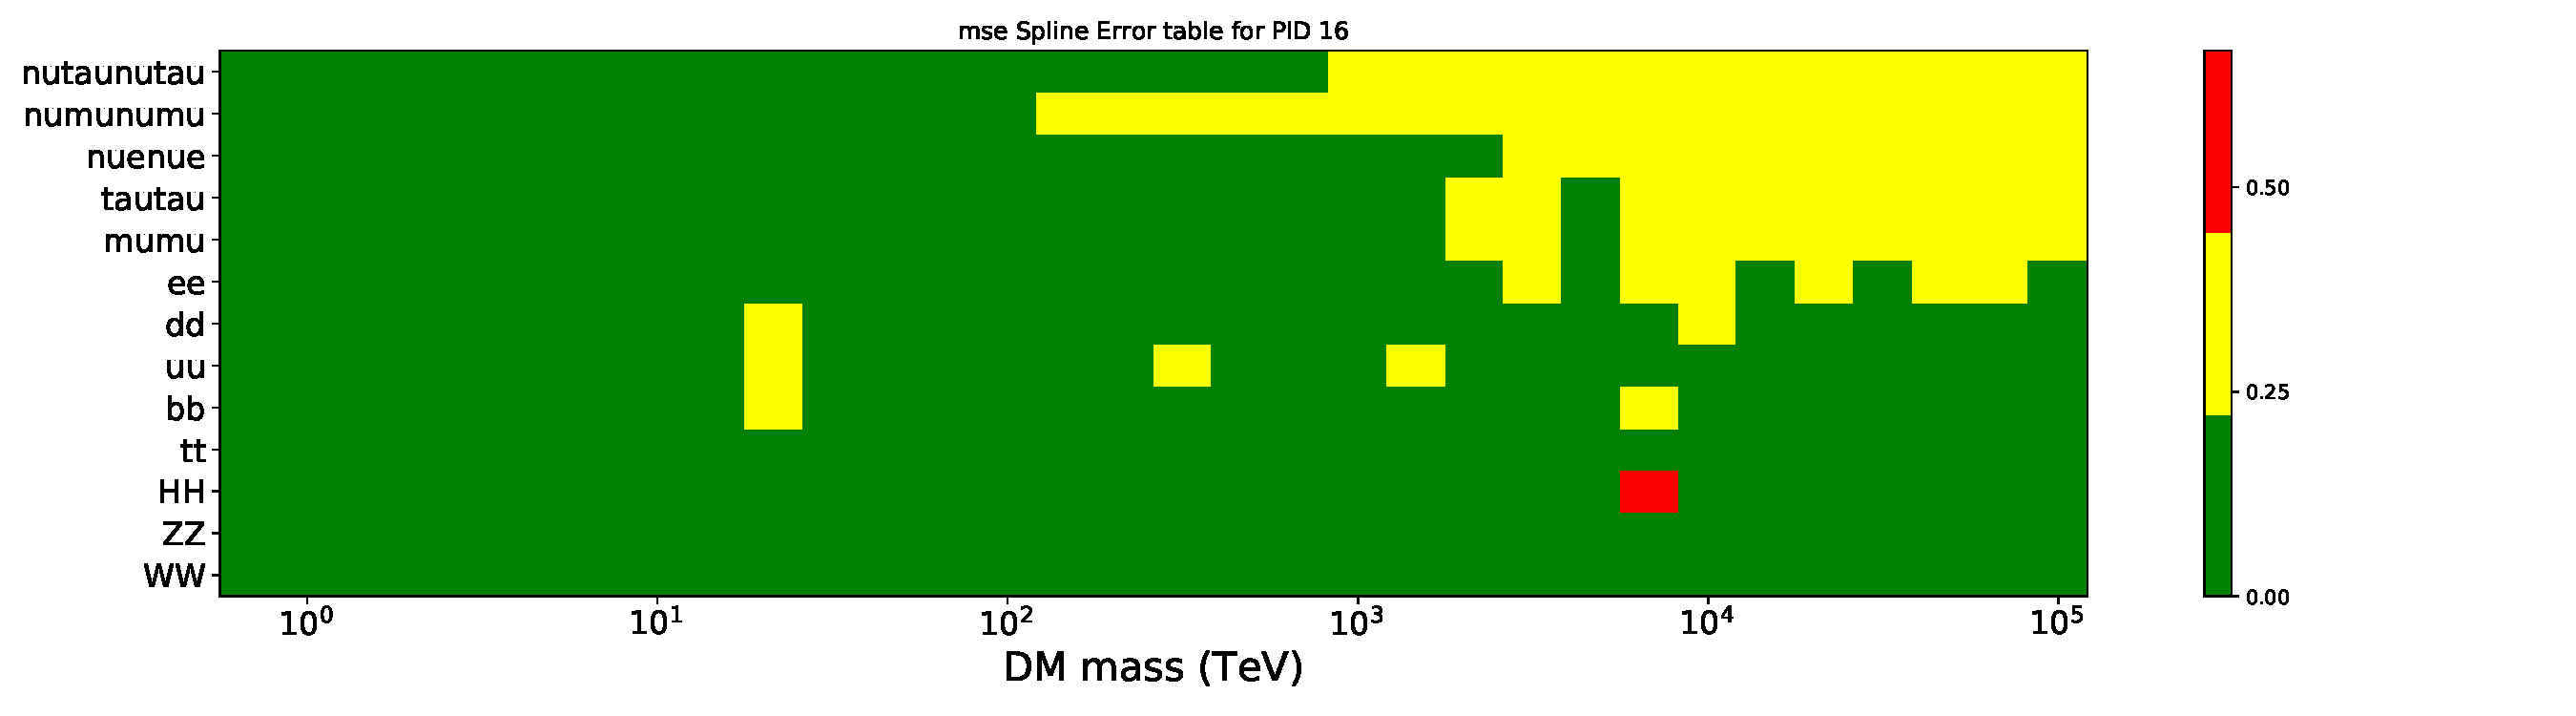
\includegraphics[scale=0.32]{figures/ic_DM/PID16_mse_error_chart.pdf}
    }
    \caption{Current status of spline tables according to contraints defined by \cref{tab:spline_tolerance}. Green splines are splines that passed under the GOOD tolerance. Yellow are splines that are OK. Red are splines that FAIL. All yellow splines were inspected individually before running the analysis. Splines were made for the $\mu$ (PID 14; top panel) flavor and $\tau$ (PID 16; bottom panel) neutrino flavors.}
    \label{fig:apdx_nu_splines}
\end{figure}

\clearpage

%%%%%%%%%%%%%%%%%%%%%%%%%%%%%%%%%%%%%%%%%%%%%%%%%%%%%%%%%%%%%
\section{Neutrino Composite Spectra} \label{sec:apdx_final_specs}
%%%%%%%%%%%%%%%%%%%%%%%%%%%%%%%%%%%%%%%%%%%%%%%%%%%%%%%%%%%%%

\begin{figure}[ht]
    \centering{
        \begin{tabular}{cc}
            $\chi\chi \rightarrow$ \parpar{b} &
            $\chi\chi \rightarrow$ \parpar{t} \\

            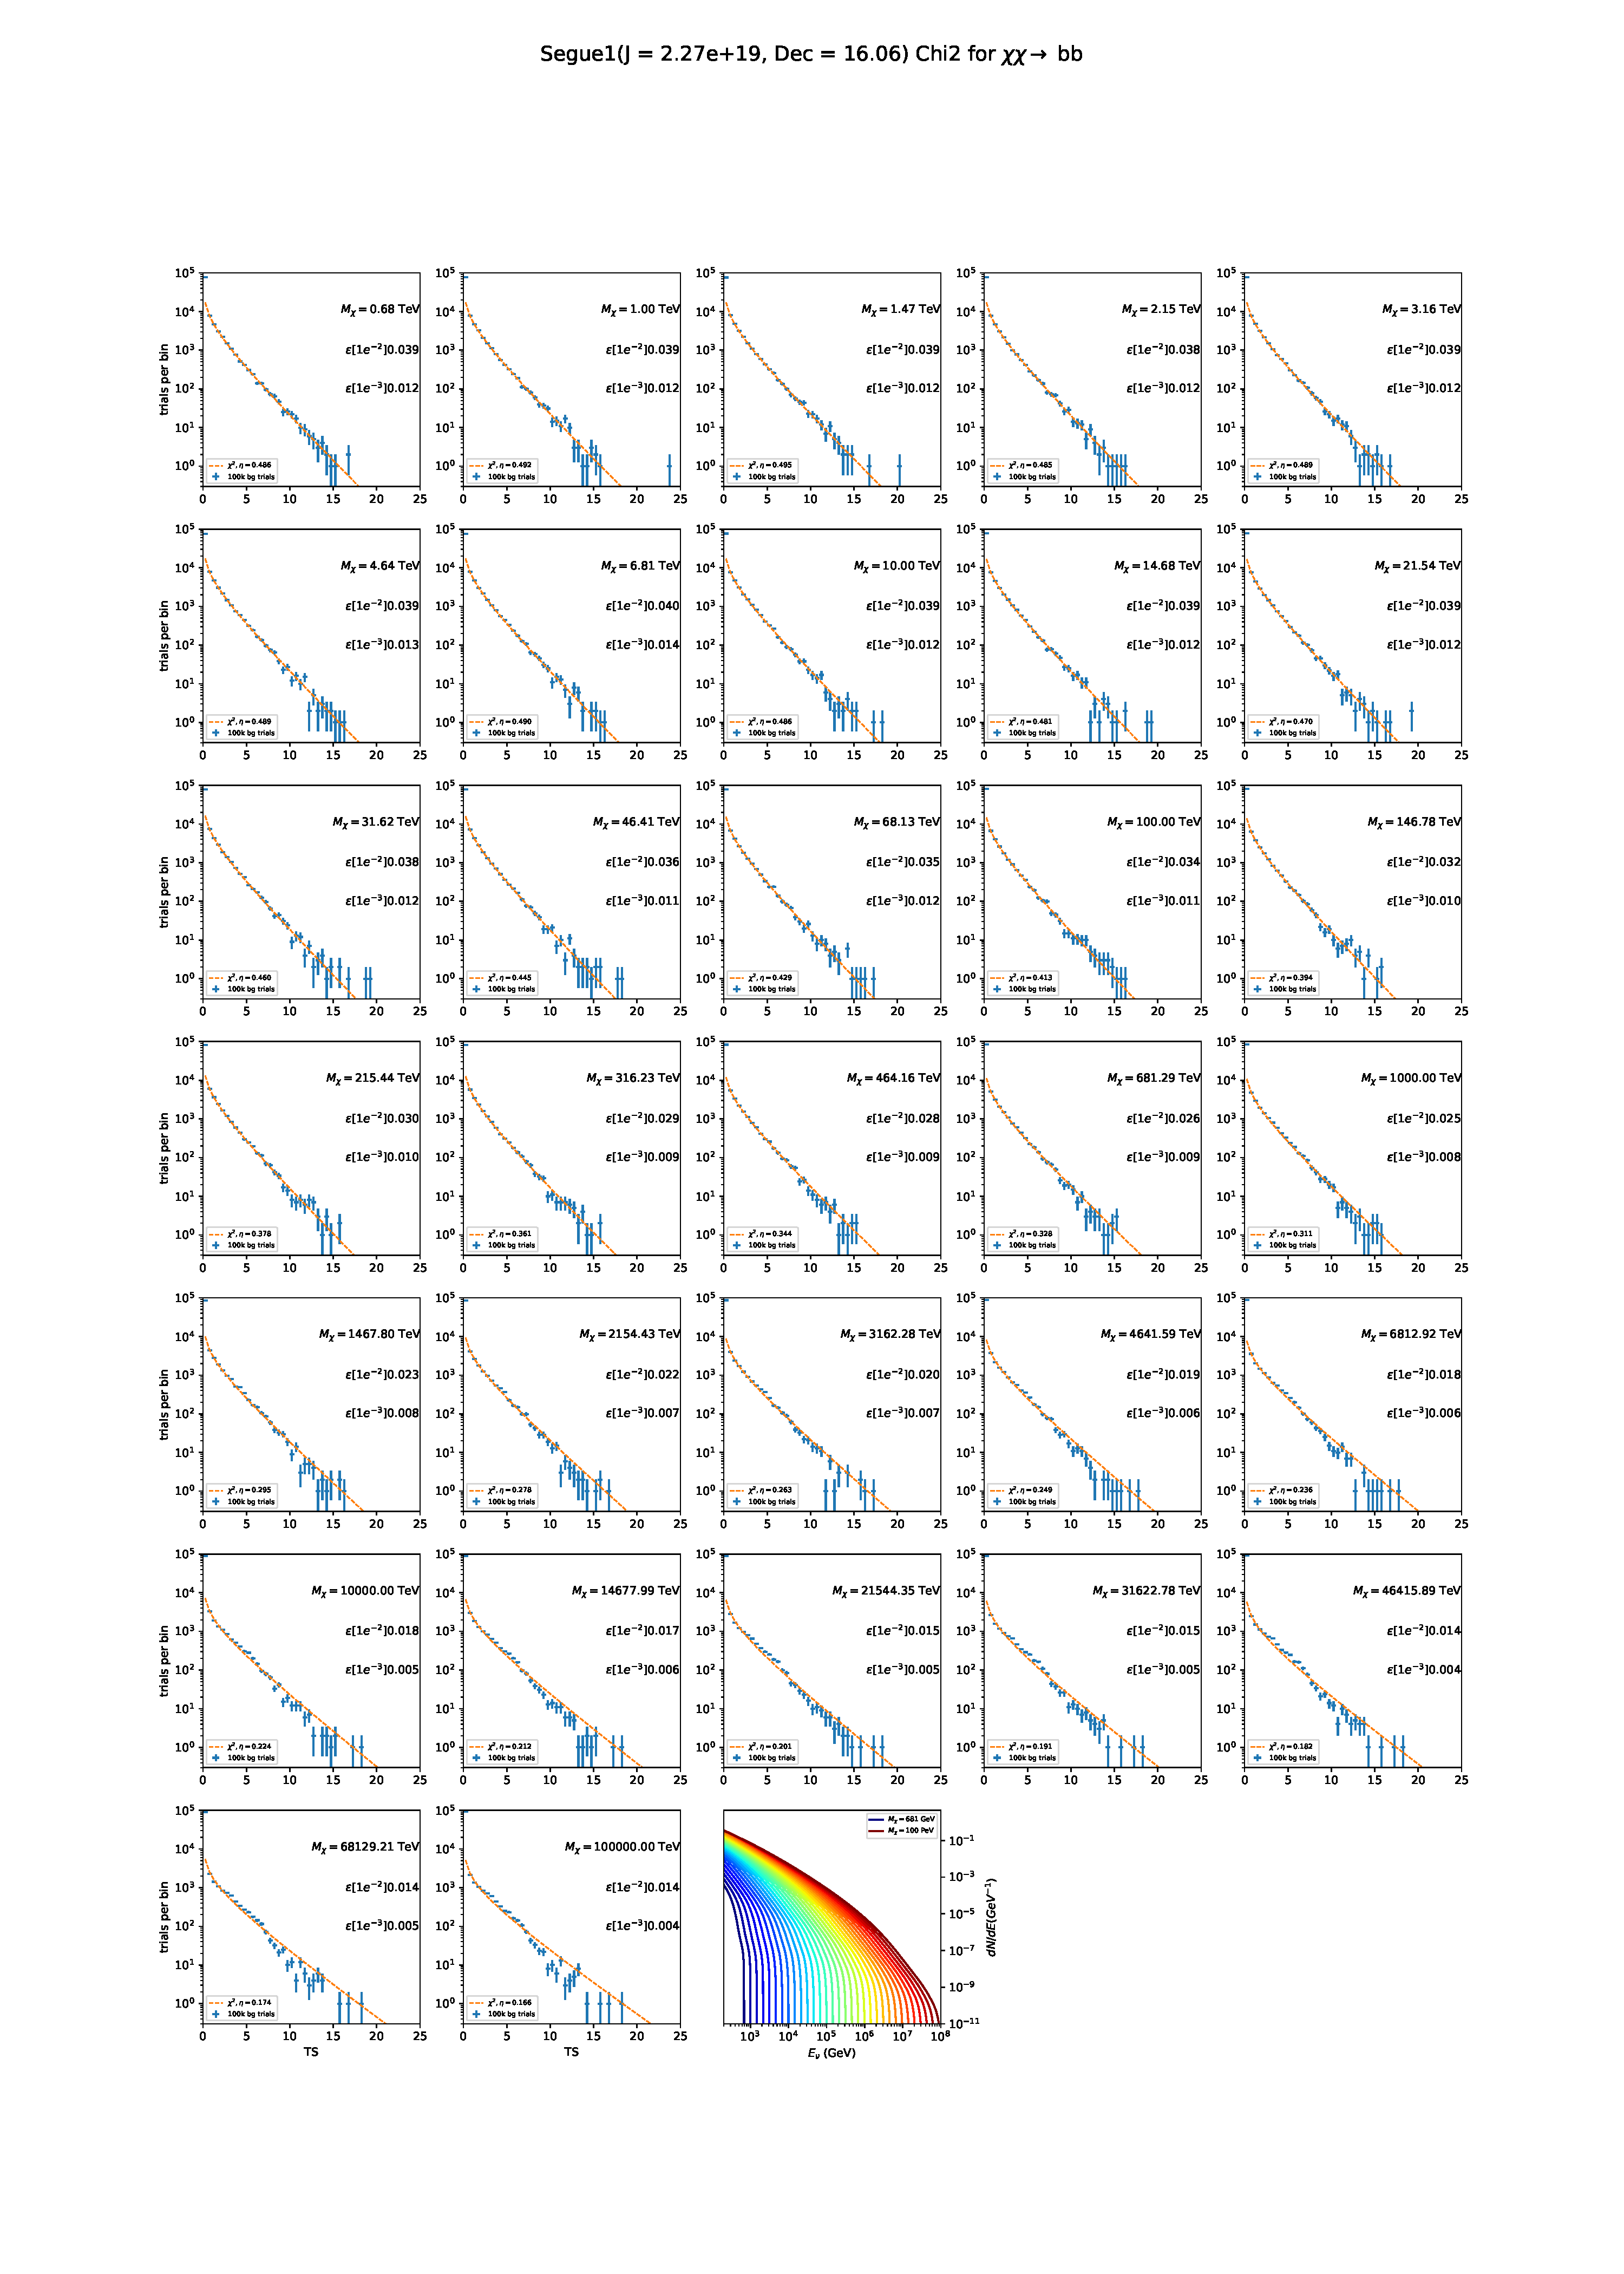
\includegraphics[clip, trim=22.1cm 6.5cm 19.5cm 56.5cm, scale=0.6]{figures/ic_DM/dm_plots/Segue1_bb_chi2_Masspanel_2024-03-23.pdf} &
            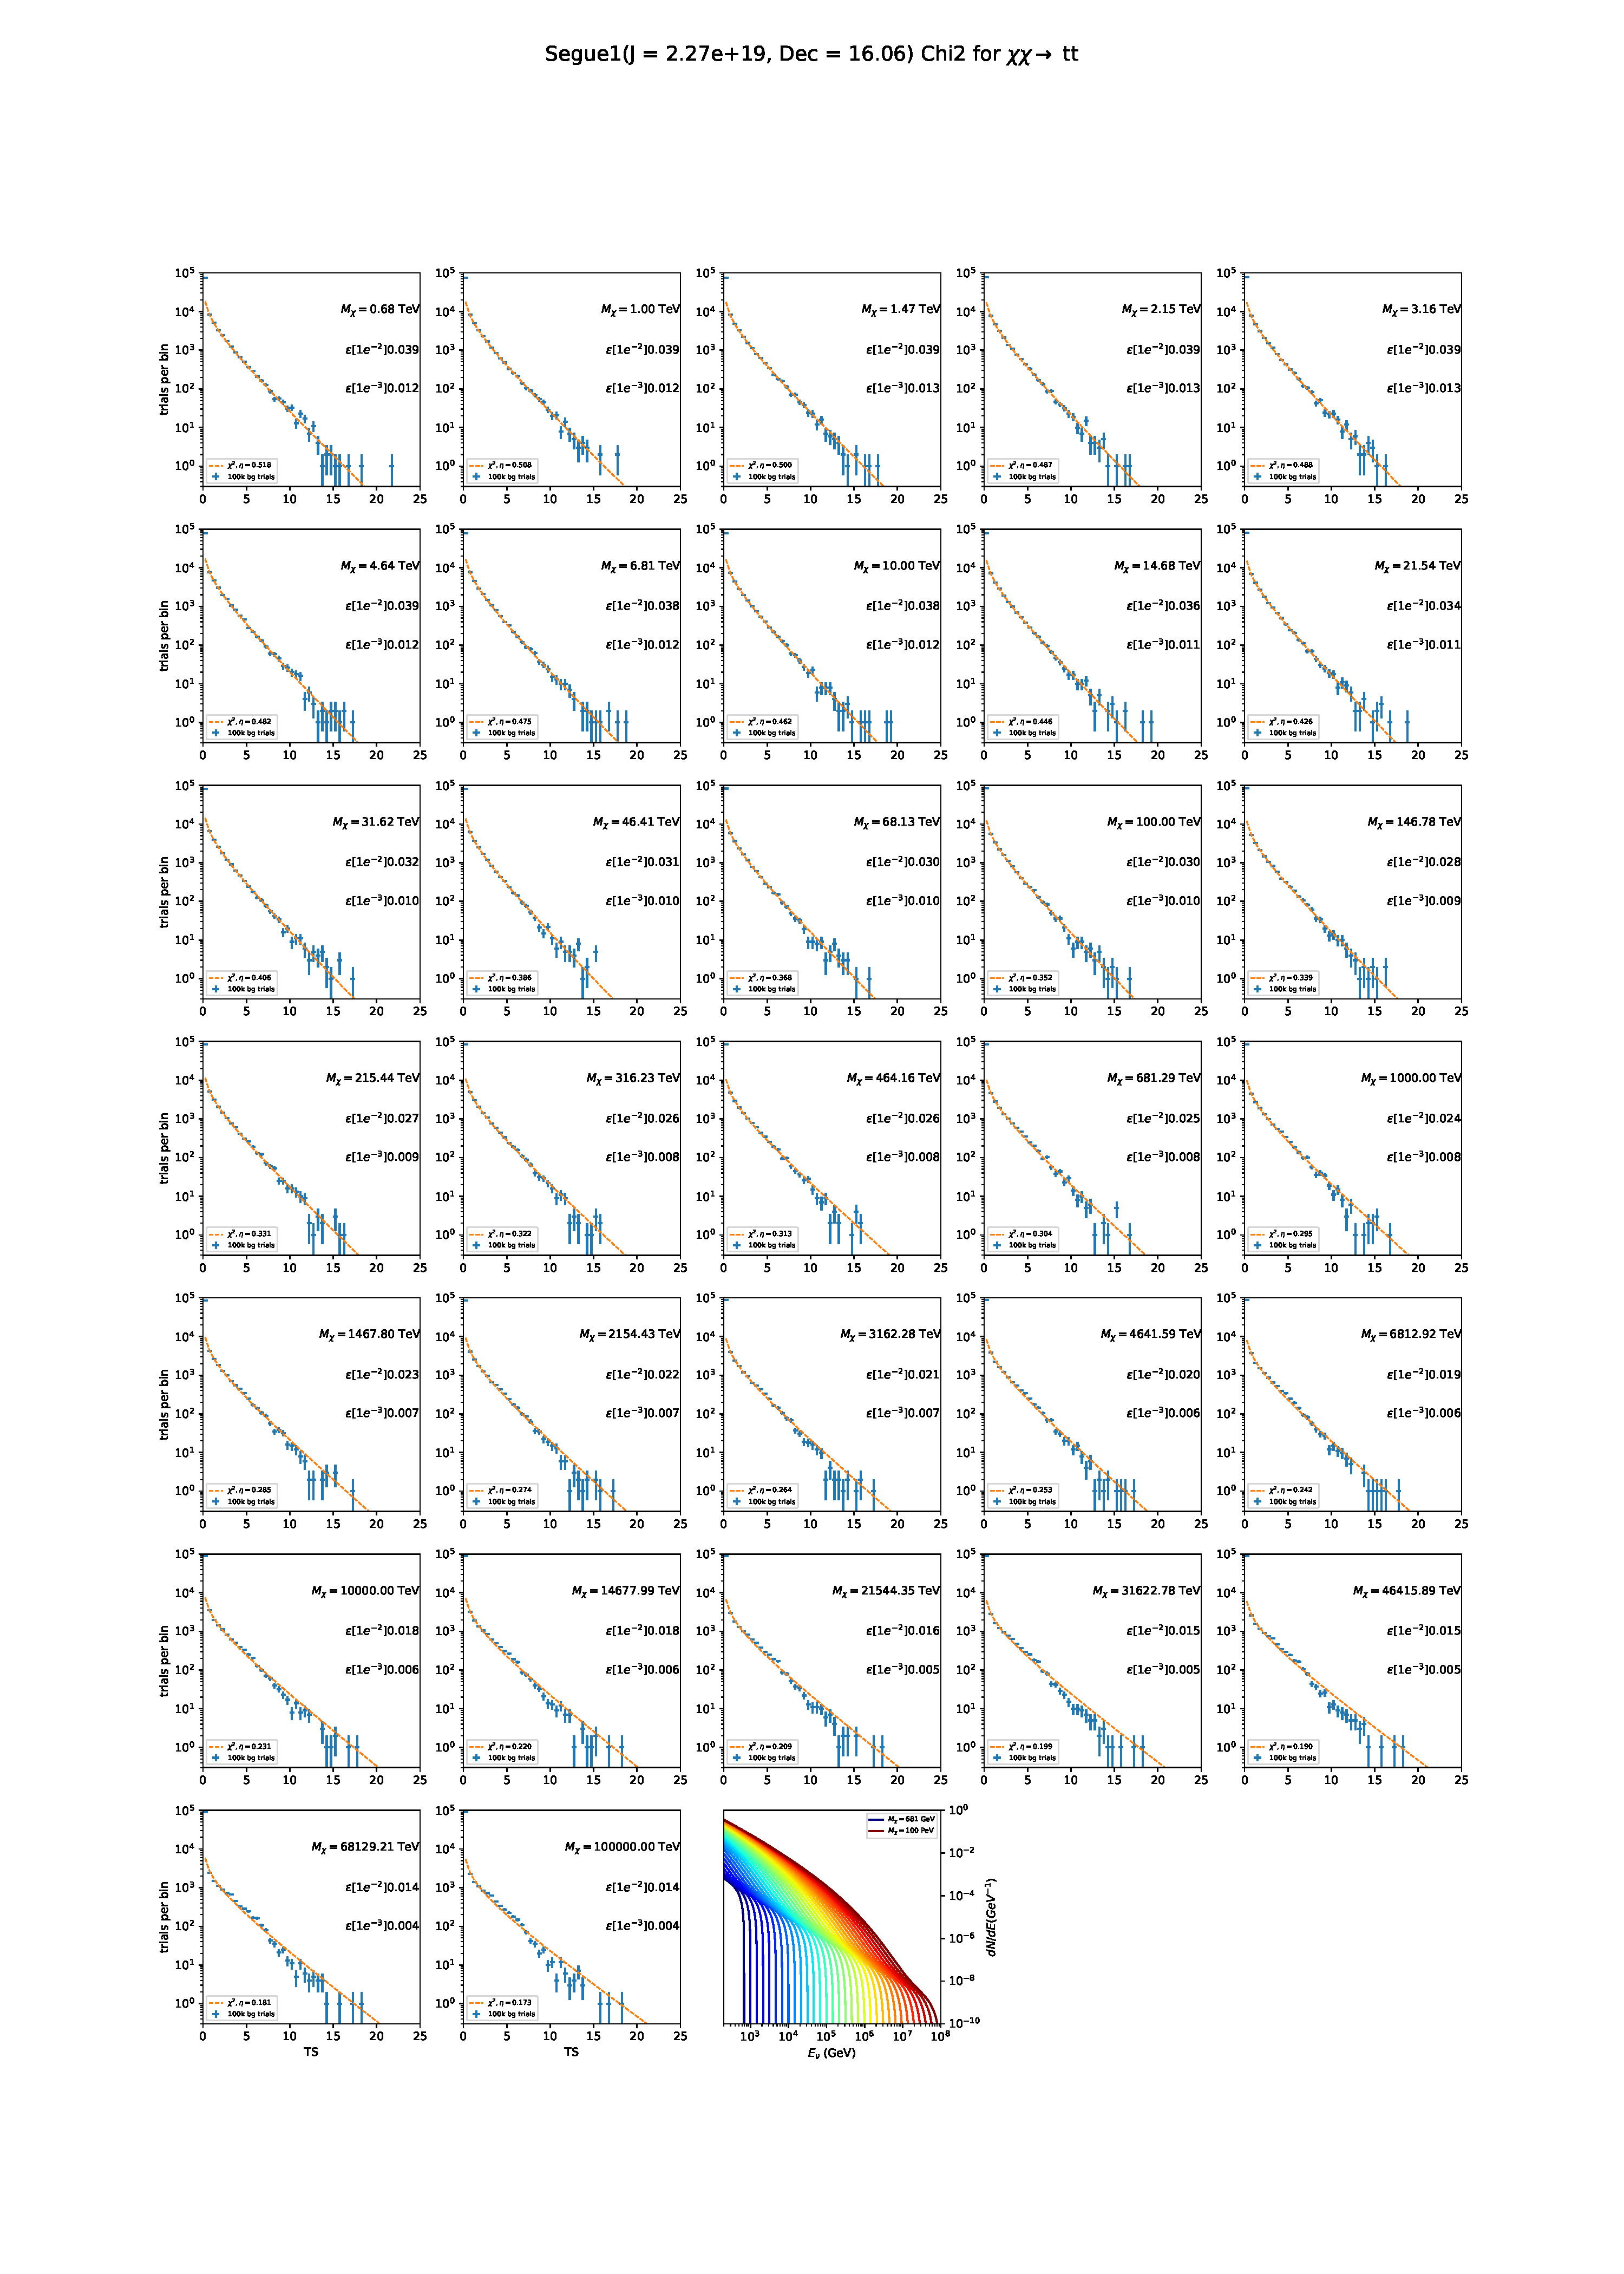
\includegraphics[clip, trim=22.1cm 6.5cm 19.5cm 56.5cm, scale=0.6]{figures/ic_DM/dm_plots/Segue1_tt_chi2_Masspanel_2024-03-23.pdf} \\

            $\chi\chi \rightarrow$ \parpar{u} &
            $\chi\chi \rightarrow$ \parpar{d} \\

            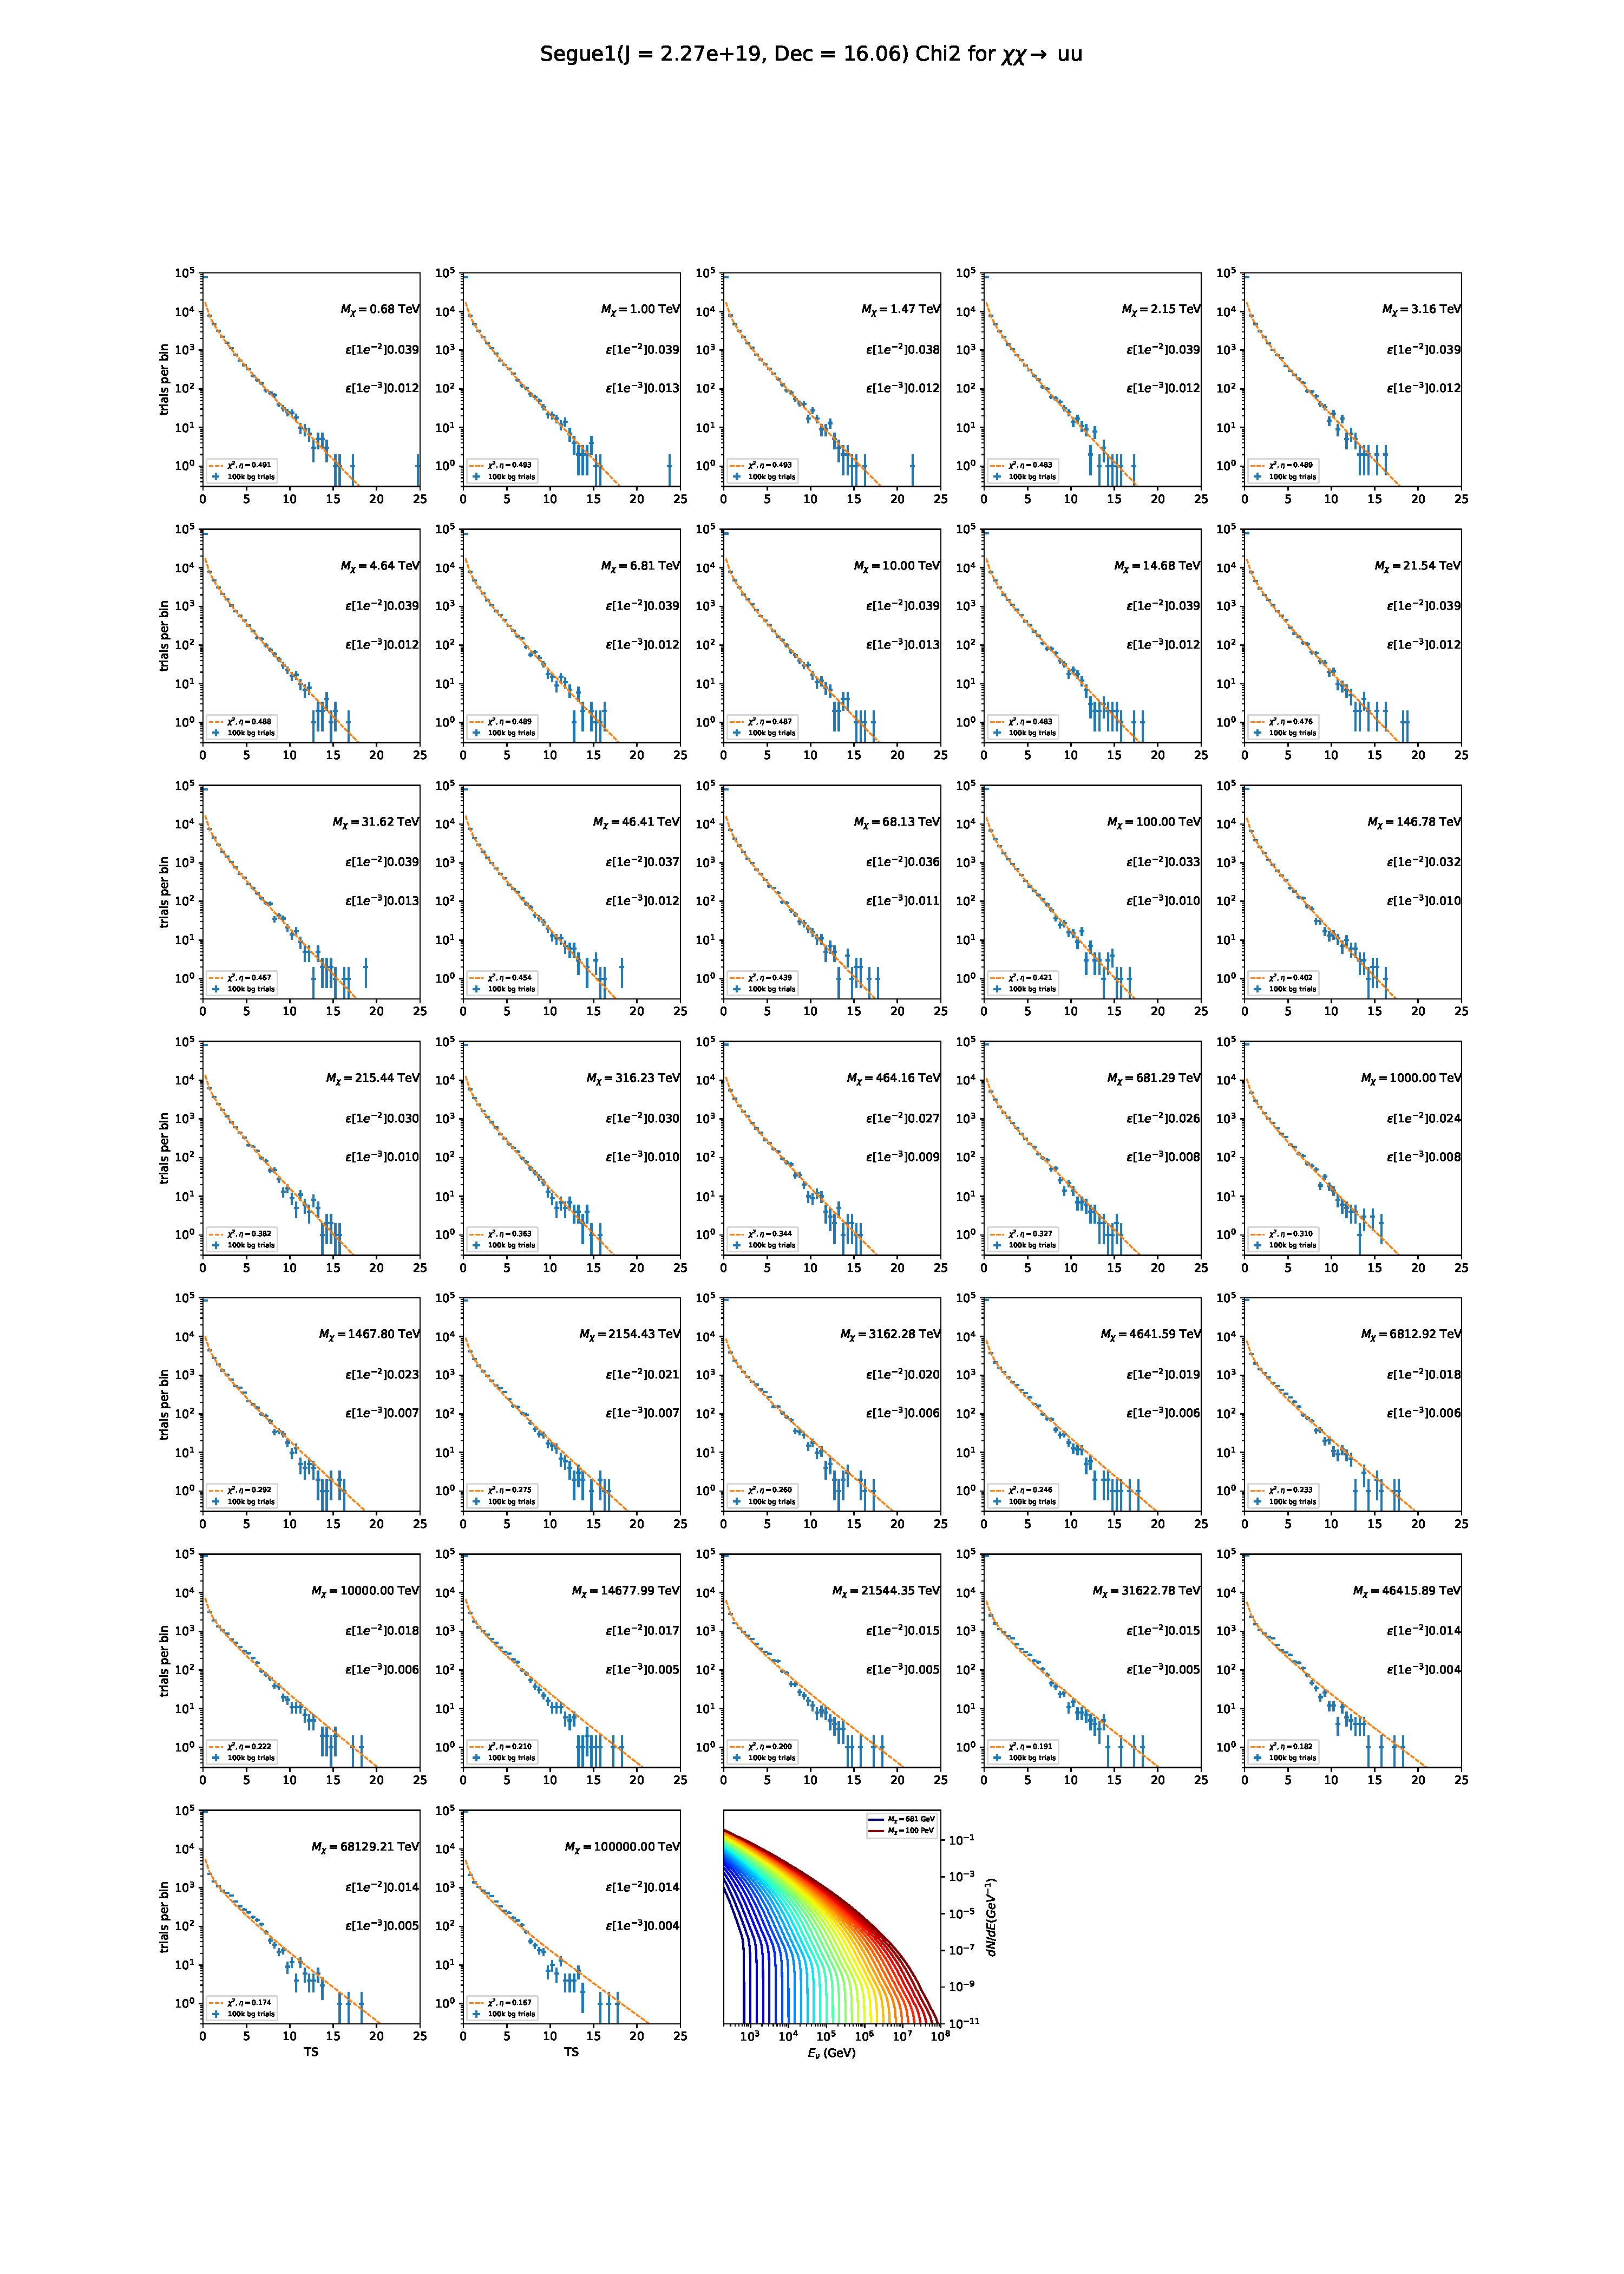
\includegraphics[clip, trim=22.1cm 6.5cm 19.5cm 56.5cm, scale=0.6]{figures/ic_DM/dm_plots/Segue1_uu_chi2_Masspanel_2024-03-23.pdf} &
            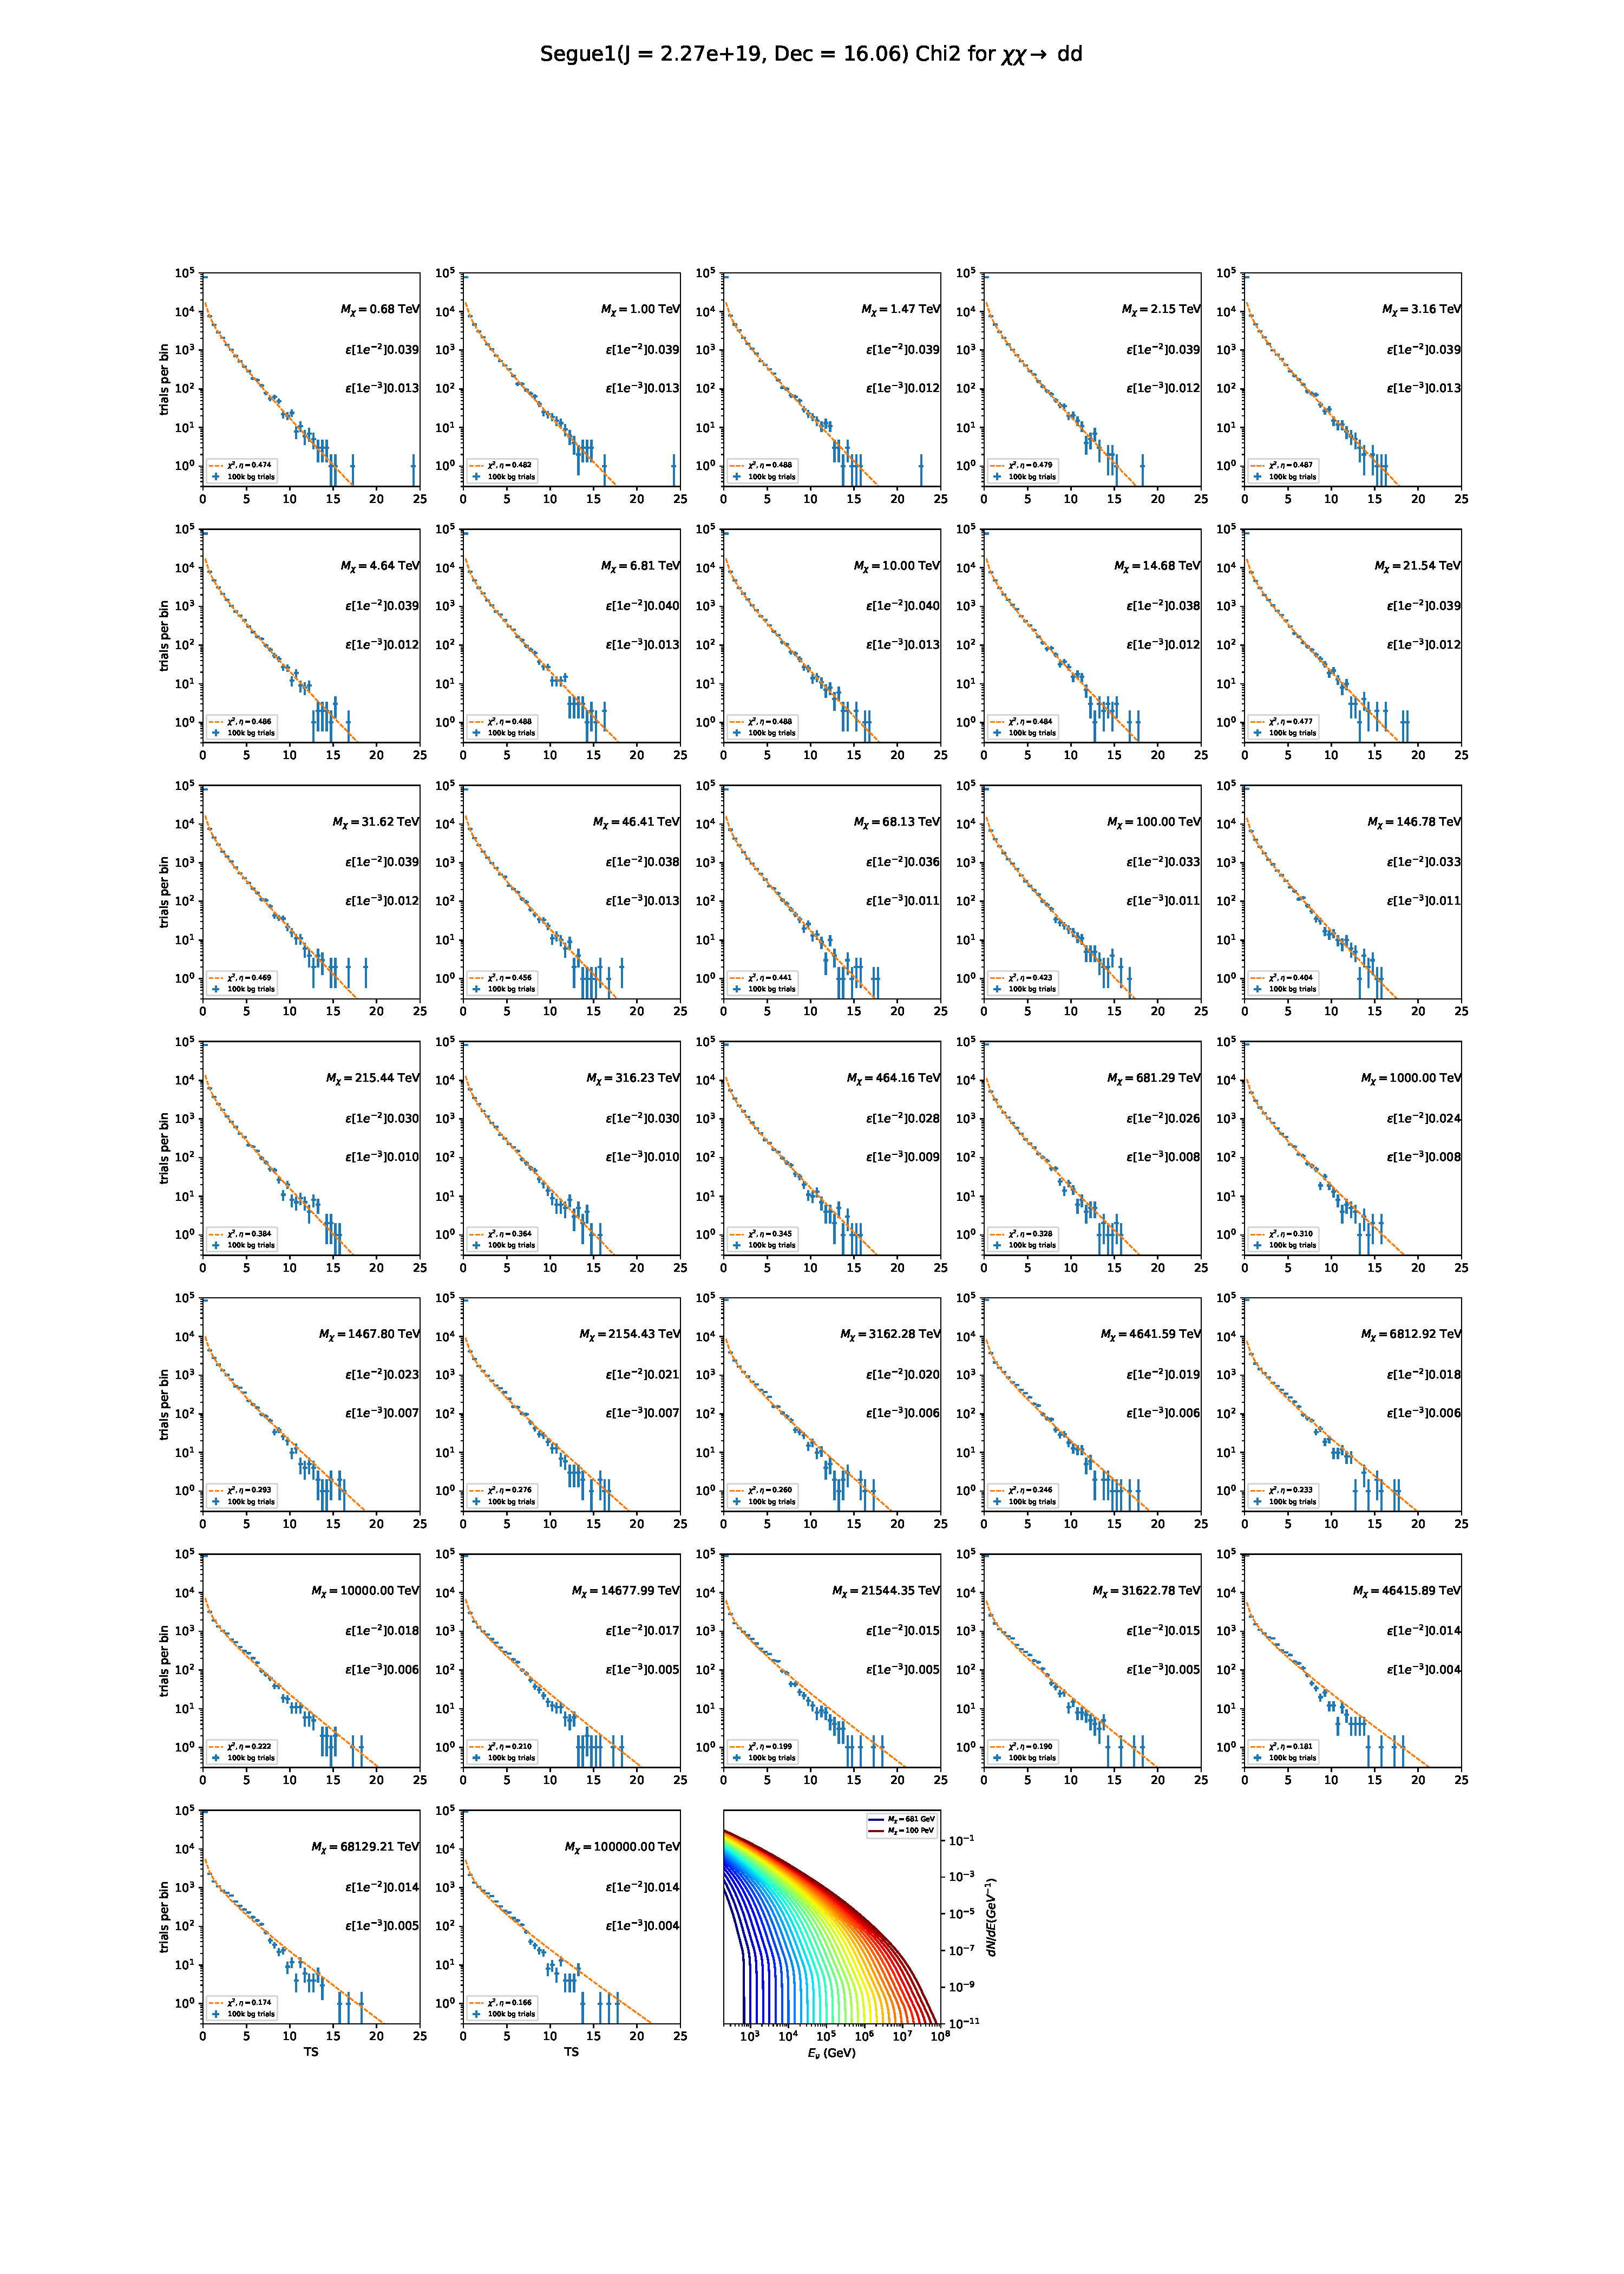
\includegraphics[clip, trim=22.1cm 6.5cm 19.5cm 56.5cm, scale=0.6]{figures/ic_DM/dm_plots/Segue1_dd_chi2_Masspanel_2024-03-23.pdf} \\

            $\chi\chi \rightarrow$ \pp{Z} &
            $\chi\chi \rightarrow$ $W^-W^+$ \\

            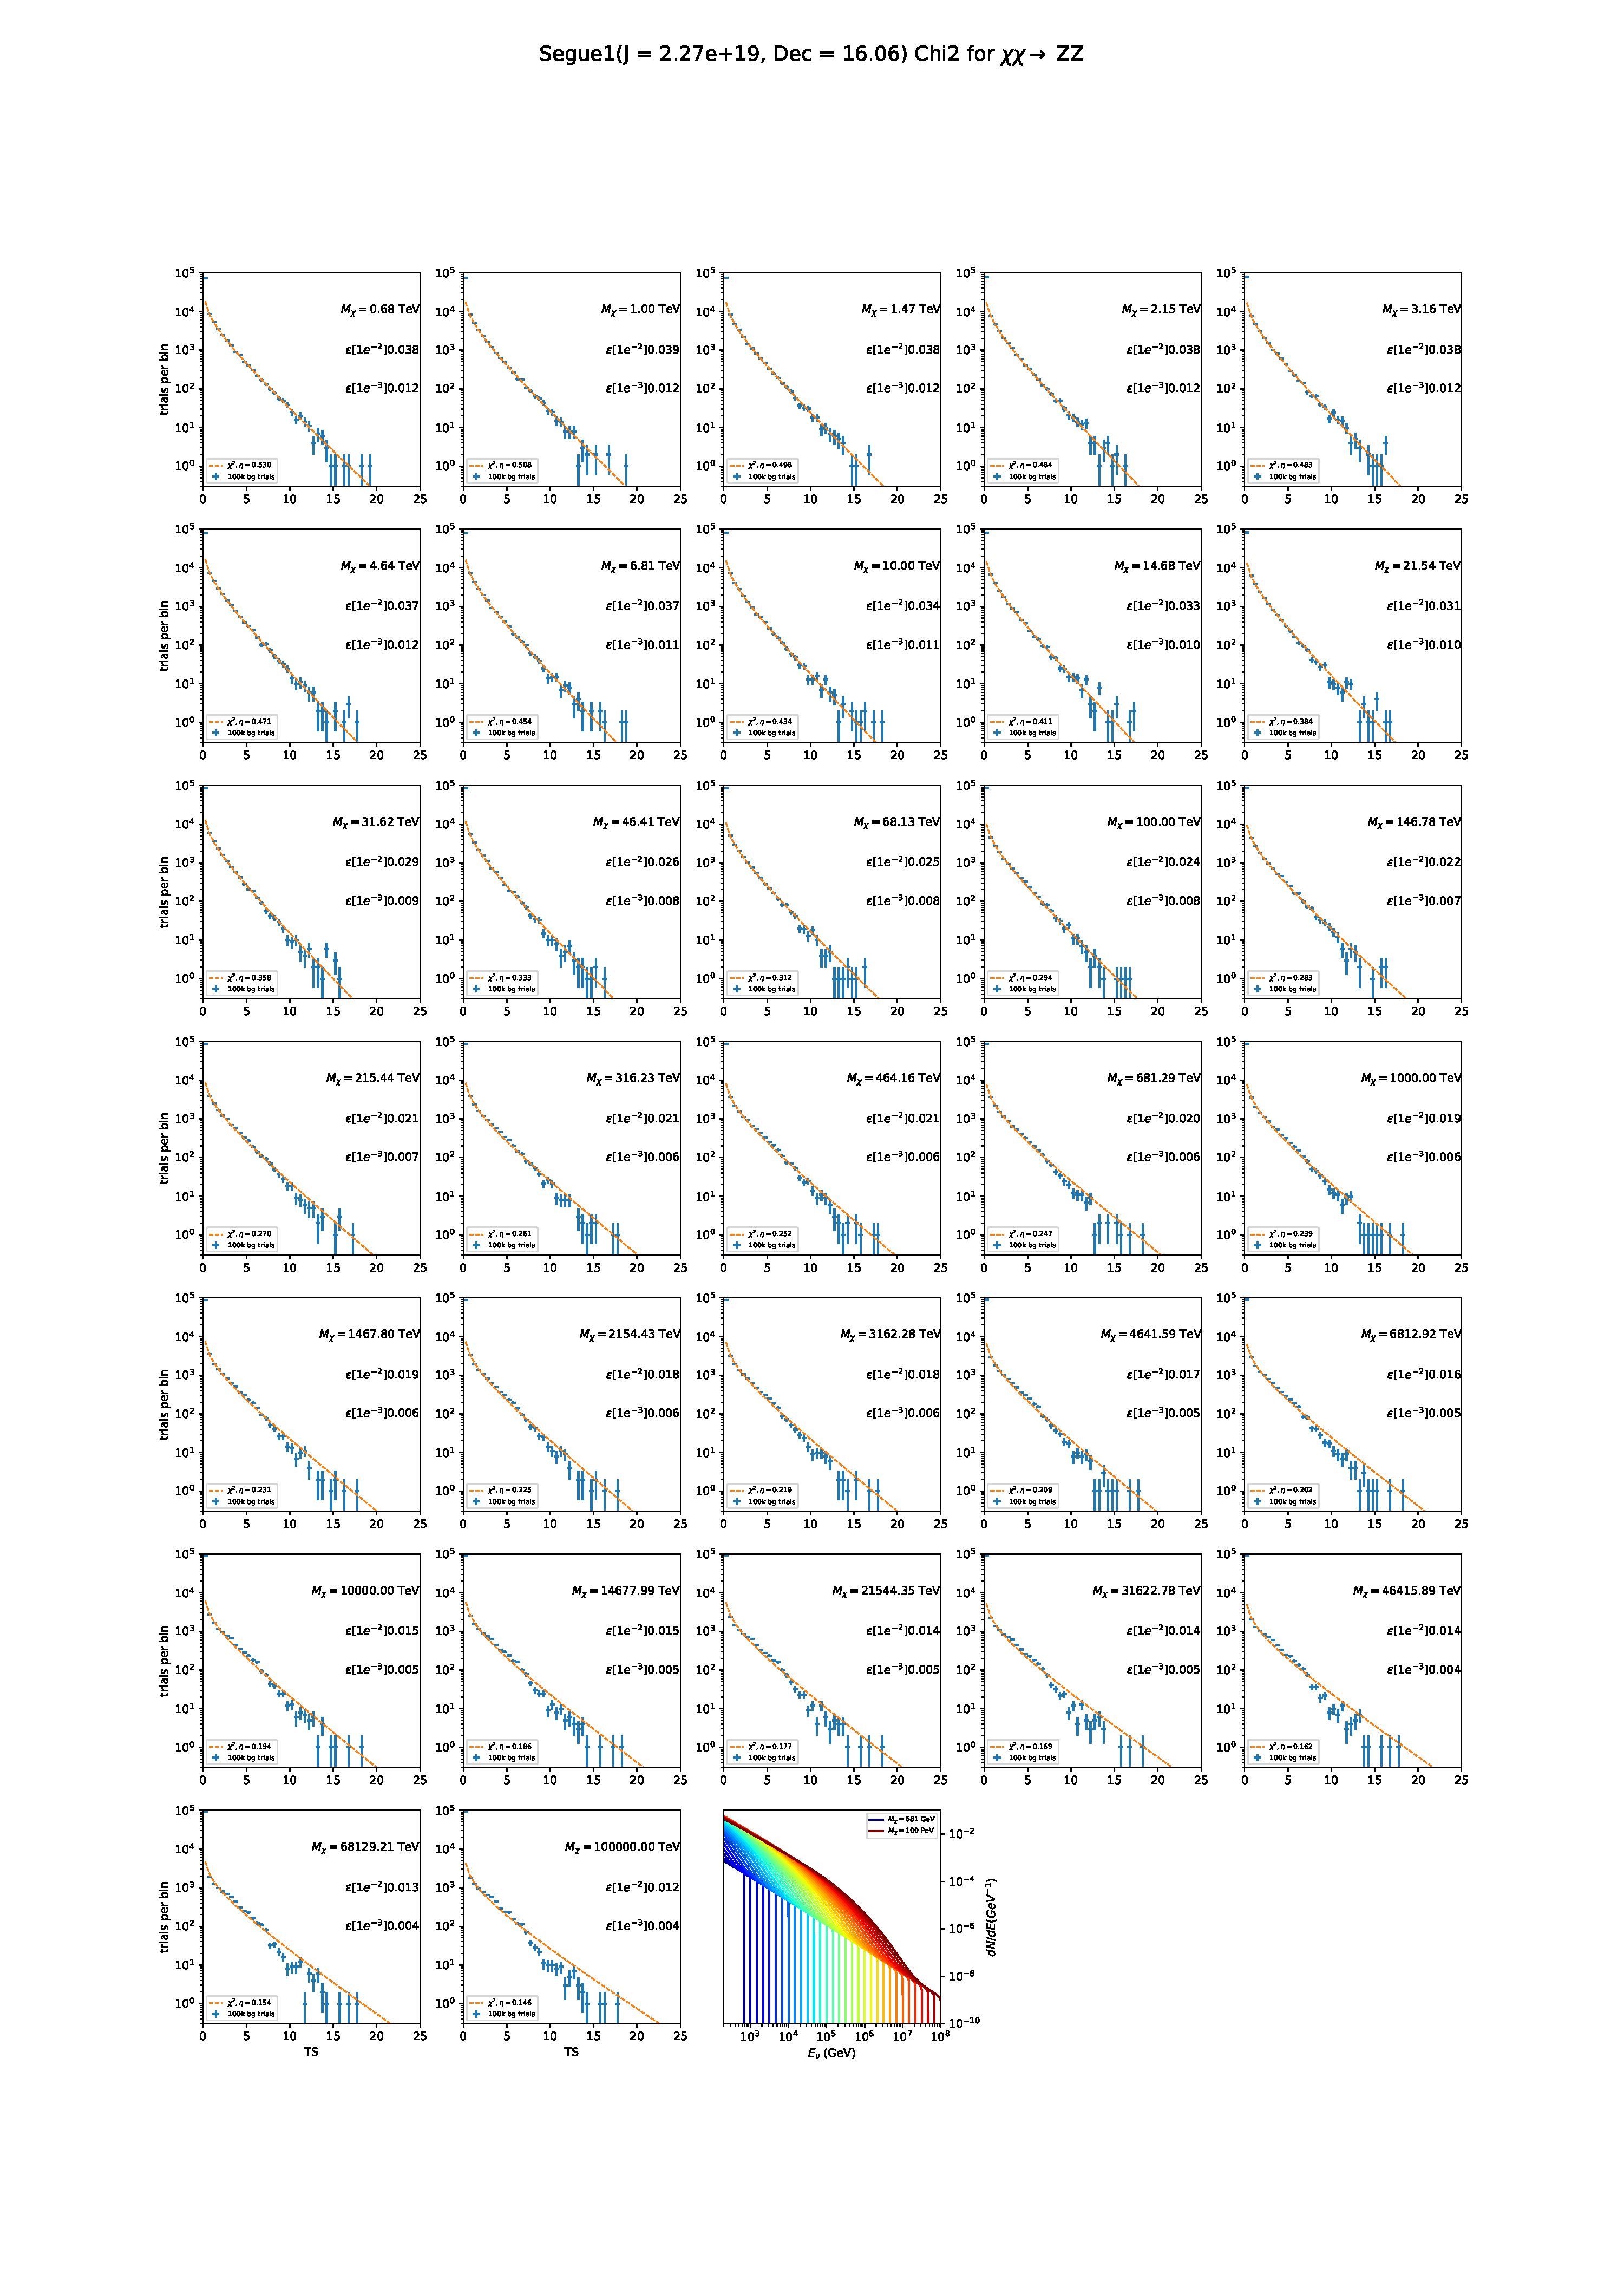
\includegraphics[clip, trim=22.1cm 6.5cm 19.5cm 56.5cm, scale=0.6]{figures/ic_DM/dm_plots/Segue1_ZZ_chi2_Masspanel_2024-03-23.pdf} &
            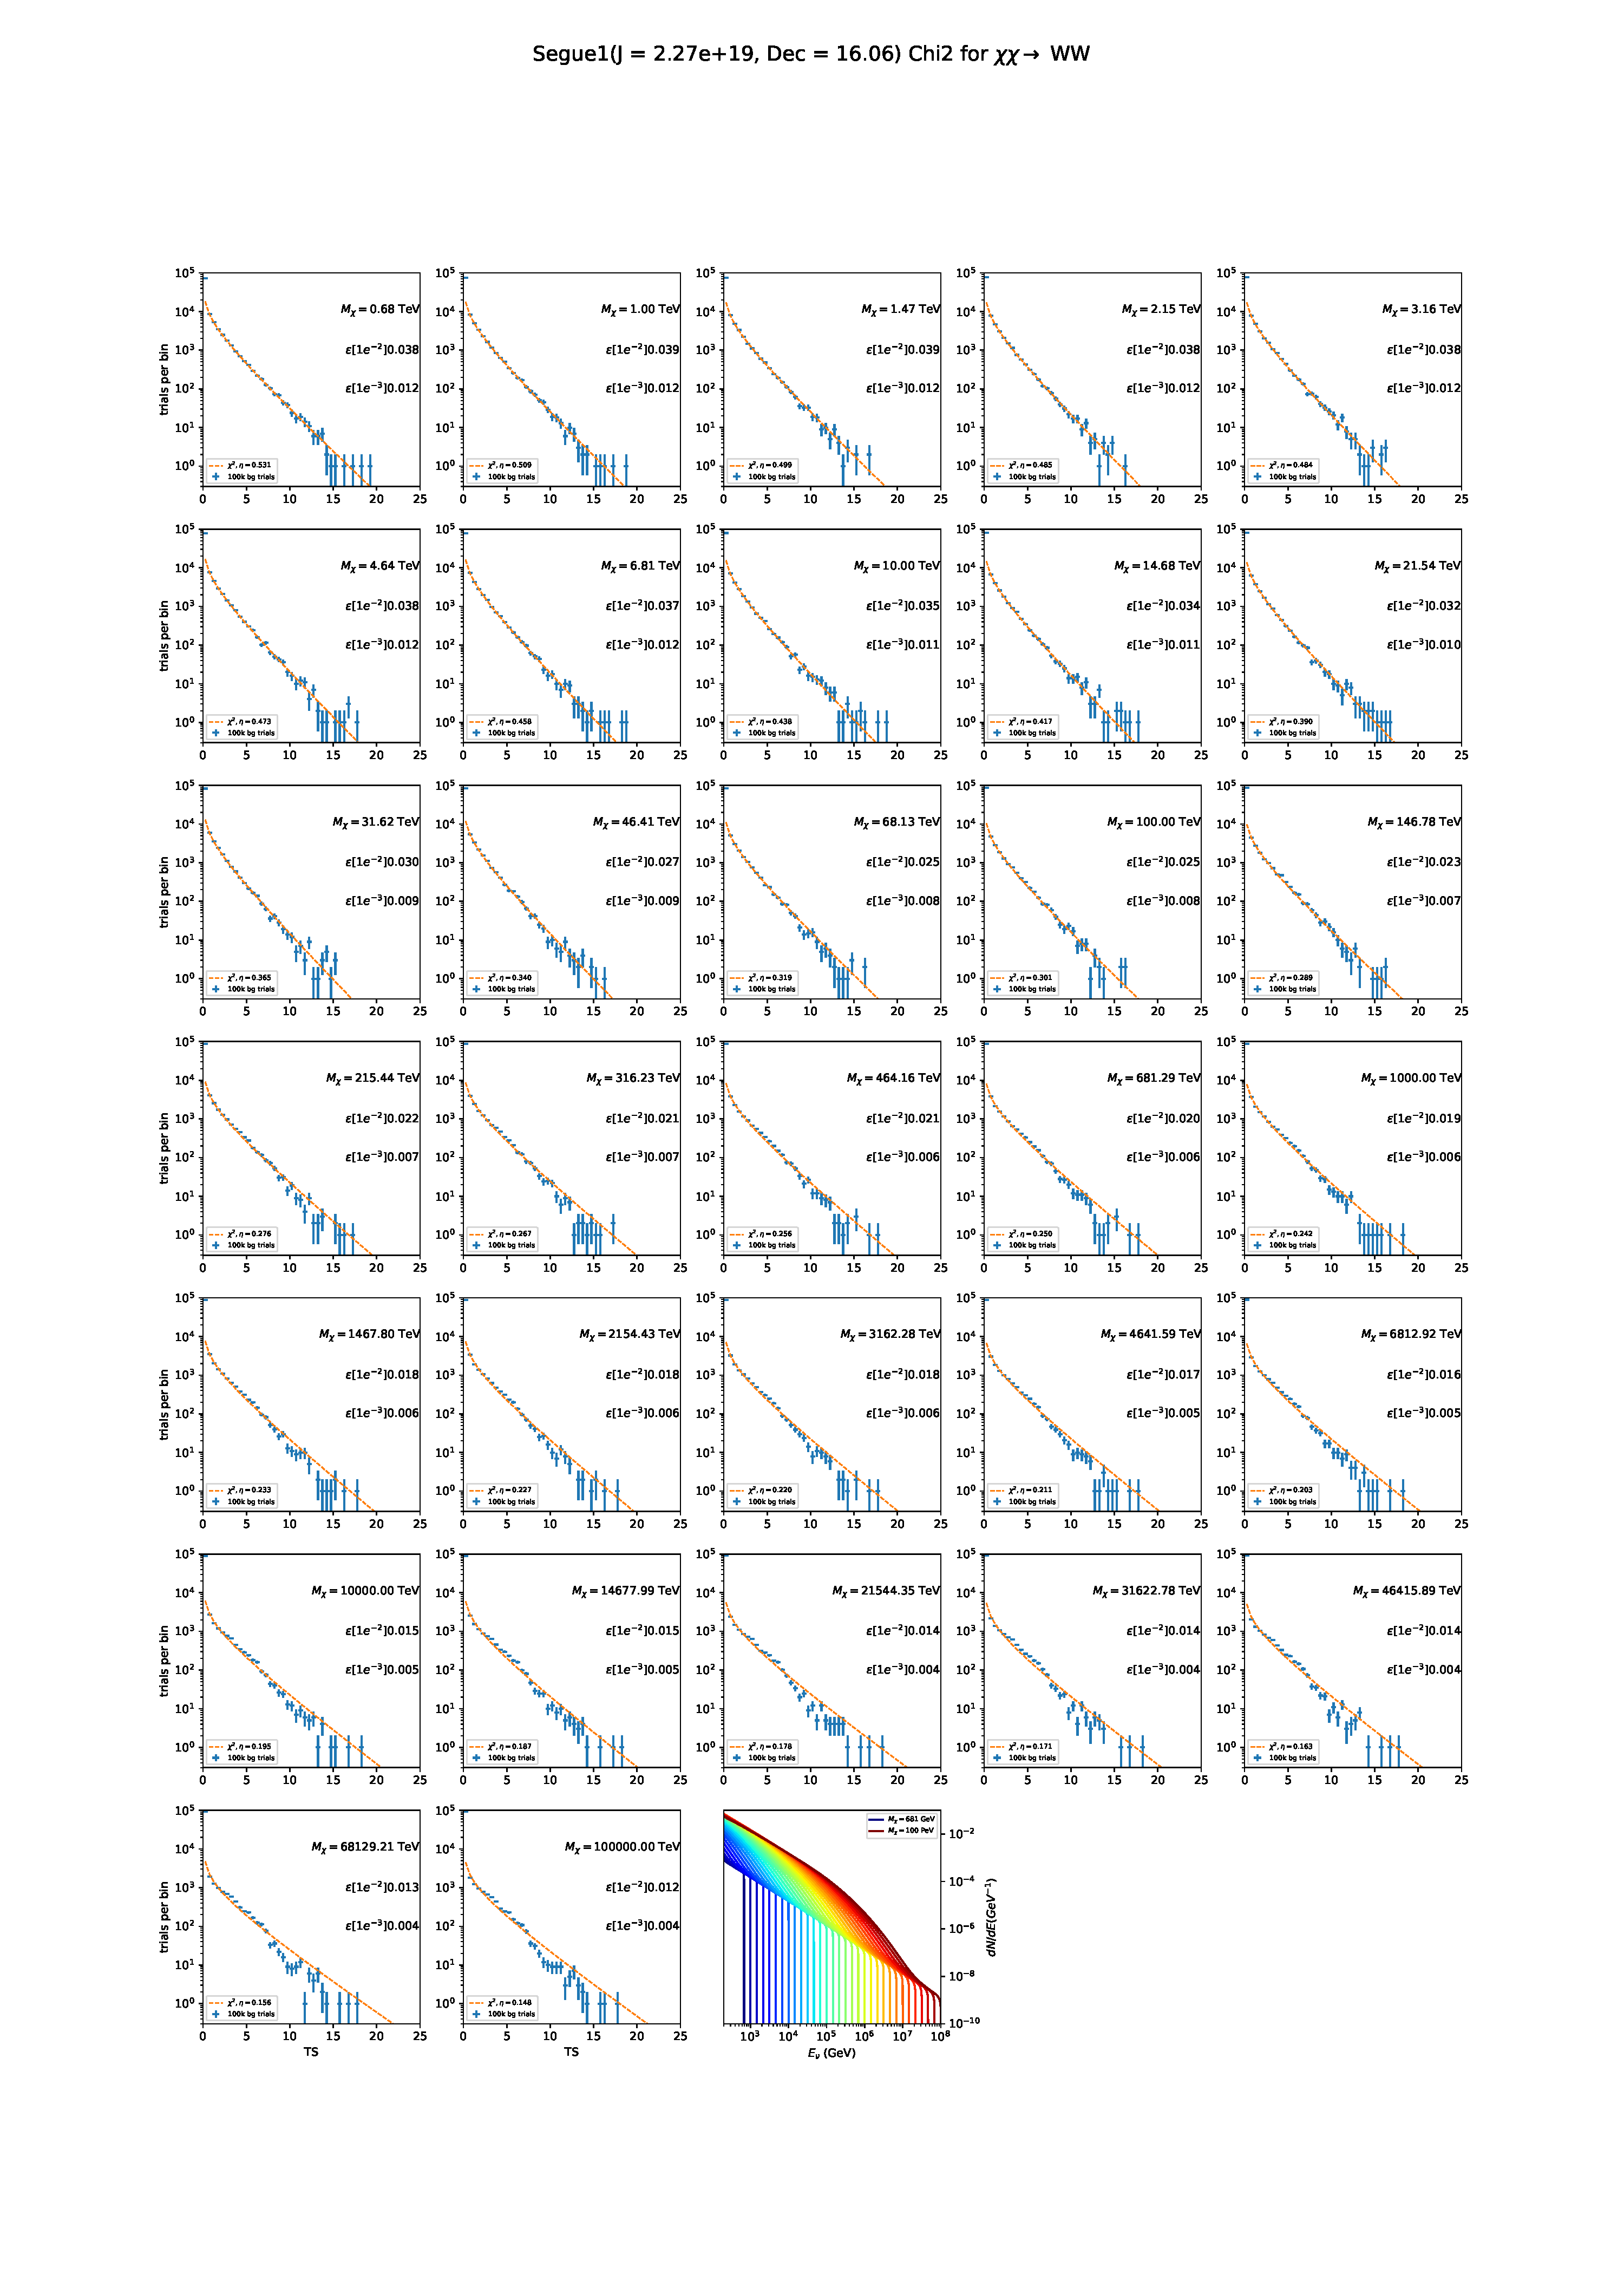
\includegraphics[clip, trim=22.1cm 6.5cm 19.5cm 56.5cm, scale=0.6]{figures/ic_DM/dm_plots/Segue1_WW_chi2_Masspanel_2024-03-23.pdf} \\
        \end{tabular}
    }\caption{Sister figure to \cref{fig:line_spectra_smooth} for annihilation channels that did not require kernel smoothing. These spectra are the composite ($\nu_\mu$ + $\nu_\tau$) of neutrino flavors. Every spectral model used for this analysis is featured as a colored solid line. Bluer lines are for lower DM mass spectral models. DM masses range from 681 GeV to 100 PeV.}
    \label{fig:compsoite_nu_spec}
\end{figure}

\clearpage

%%%%%%%%%%%%%%%%%%%%%%%%%%%%%%%%%%%%%%%%%%%%%%%%%%%%%%%%%%%%%
\section{Segue 1 And Ursa Major II Signal Recovery} \label{sec:apdx_TS_per_src}
%%%%%%%%%%%%%%%%%%%%%%%%%%%%%%%%%%%%%%%%%%%%%%%%%%%%%%%%%%%%%
 \tmpfig{Fill this out eventually. I think I want all the plots generated first}